%\subsubsection{Konzept ( Warum muss man invertieren? )}

%Das Lochkamera-Modell geht von einer infinitesimal kleinen Blendenöffnung aus. Einfallende Lichtstrahlen, die auf die Öffnung treffen, bewegen sich ungehindert in ihre Ausbreitungsrichtung weiter und treffen an einem Punkt $p_1$ auf den Kamerasensor (siehe blauer Strahl in Abbildung \ref{fig:model}).
Die Auswirkungen einer Linsenverzerrung sind in Abbildung \ref{fig:model} dargestellt. Der Lichtstrahl bewegt sich nicht mehr ungehindert in seiner Ausbreitungsrichtung weiter und trifft an einem Punkt $p_1$ auf den Kamerasensor (siehe blauer Strahl), sondern
wird an der Öffnung der Lochblende in einem bestimmten Maße abgeknickt und erreicht den Sensor am Punkt $p_2$ (roter Strahl). Die Funktion, die die normalisierten Pixelkoordinaten des unverzerrten Punktes $p_1$ auf die des verzerrten Punktes $p_2$ abbildet, bezeichnen wir mit $f$.
\begin{figure}[h]
	\centering
	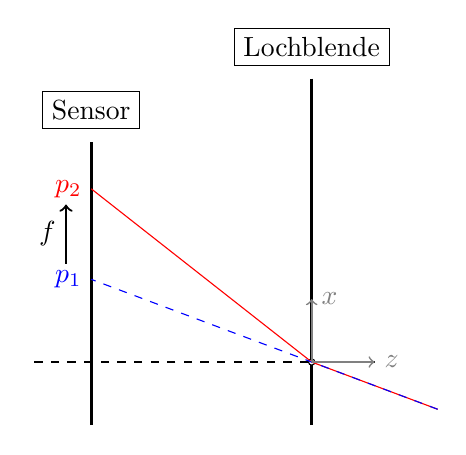
\begin{tikzpicture}[scale=0.4]

	% sensor
	\draw[very thick] (-7,-2) -- (-7, 7);
	% lochblende
	\draw (0,0) circle [radius=0.1];
	\draw[very thick] (0, -2) -- (0, -0.1);
	\draw[very thick] (0, 9) -- (0, 0.1);
	%optische Achse
	\draw[thin, dashed] (2, 0) -- (-9, 0);
	%abgelenkter Lichtstrahl
	\draw[red] (4, -1.5) -- (0, 0) -- (-7, 5.5) node[left] {$p_2$};
	%durchgehender Lichtstrahl
	\draw[blue, dashed] (4, -1.5) -- (-7, 21/8) node[left] {$p_1$};
	%Verzeichnungspfeil
	\draw[->, thick] (-7.8, 21/8 + 0.5) -- (-7.8, 65/16) node[left] {$f$} -- (-7.8, 5) ;
	%Koordinatensystem
	\draw[semithick, gray, ->] (0,0) -- (0,2) node[right] {$x$};
	\draw[semithick, gray, ->] (0,0) -- (2,0) node[right] {$z$};
	%Beschriftung
	\node[draw] at (-7, 8) {Sensor};
	\node[draw] at (0, 10) {Lochblende};
	\end{tikzpicture}
	\caption{Vereinfachtes Verzerrungsmodell in 2D. Der rote von rechts einfallende Lichtstrahl wird durch die Linse abgelenkt. In blau ist der Weg dargestellt, den der Strahl nach dem Lochkamera-Modell nehmen würde. Die gestrichelte Linie zeigt die optische Achse. Die Abbildung zwischen Lochkamera-Modell und Modell mit Verzerrung ist mit $f$ bezeichnet.}
	\label{fig:model}
\end{figure}
Ein Raytracer, der eine solche Linsenverzerrung berücksichtigen soll, muss also bei der Erzeugung der Strahlen für einen gegebenen Punkt von dem Lochkamera-Modell aus Abschnitt \ref{sec:pinhole} abweichen.

 Allerdings gibt es für jeden Punkt $p$ auf dem Sensor einen Punkt $p'$, deren zugeordneter Strahl für $z\ge0$ \emph{nach dem Lochkamera-Modell} dem Strahl entspricht, der \emph{nach dem Verzerrungsmodell} $p$ zuzuordnen ist.
In Abbildung \ref{fig:model} ist $p = p_2$ und $p' = p_1$. Da $f(p_1) = p_2$ ist, kann damit $p'$ durch Anwenden der inversen Verzerrungsfunktion $g = f^{-1}$ mit $p' = g(p)$ gefunden werden. Der Strahl für $p$ kann dann einfach nach dem Lochkamera-Modell berechnet werden, indem $p = p'$ gesetzt wird.
